\chapter{Termodinâmica estatística aplicada}\label{ch:b3:statistical-thermo-applied}

O hidrogênio líquido guardado no tanque mais bem isolado continua a evaporar
e, nos primeiros dias depois da liquefação, evapora muito mais depressa do que
o calor que entra pelas paredes consegue explicar. O calor vem de dentro do
líquido. As moléculas de hidrogênio existem em duas formas, que diferem apenas
pela orientação relativa dos spins de seus dois prótons e que se convertem uma
na outra muito lentamente; a \qty{20}{K}, a conversão de uma forma na outra
libera mais calor do que o necessário para evaporar o líquido. Este capítulo
aplica as funções de partição do \cref{ch:b3:partition-functions} às
capacidades caloríficas, a esses isômeros de spin nuclear e à entropia que
certos cristais conservam a 0 K, e depois calcula constantes de equilíbrio e
efeitos isotópicos apenas a partir de dados espectroscópicos.

\begin{recall}
O \cref{ch:b3:partition-functions} construiu a \omterm{def:b3:partition-functions:partition-function}{função de partição molecular} e
seus quatro fatores, e deduziu dela $U$, $S$ e $G$. O volume do 2.º ano
relacionou a constante de equilíbrio padrão à energia de Gibbs padrão de reação,
$\Delta_rG^\circ = -RT\ln K^\circ$, e estabeleceu a equação de van 't Hoff; o
\cref{ch:b3:many-electron-atoms} afirmou que uma função de onda muda de sinal
quando dois férmions idênticos são permutados; o
\cref{ch:b3:rovibrational-spectroscopy} encontrou a alternância 3:1 das
intensidades das raias no espectro Raman rotacional de moléculas como \ce{H2}. A
parte do 9.º ano do volume escolar definiu os isótopos.
\end{recall}

\begin{omfigure}
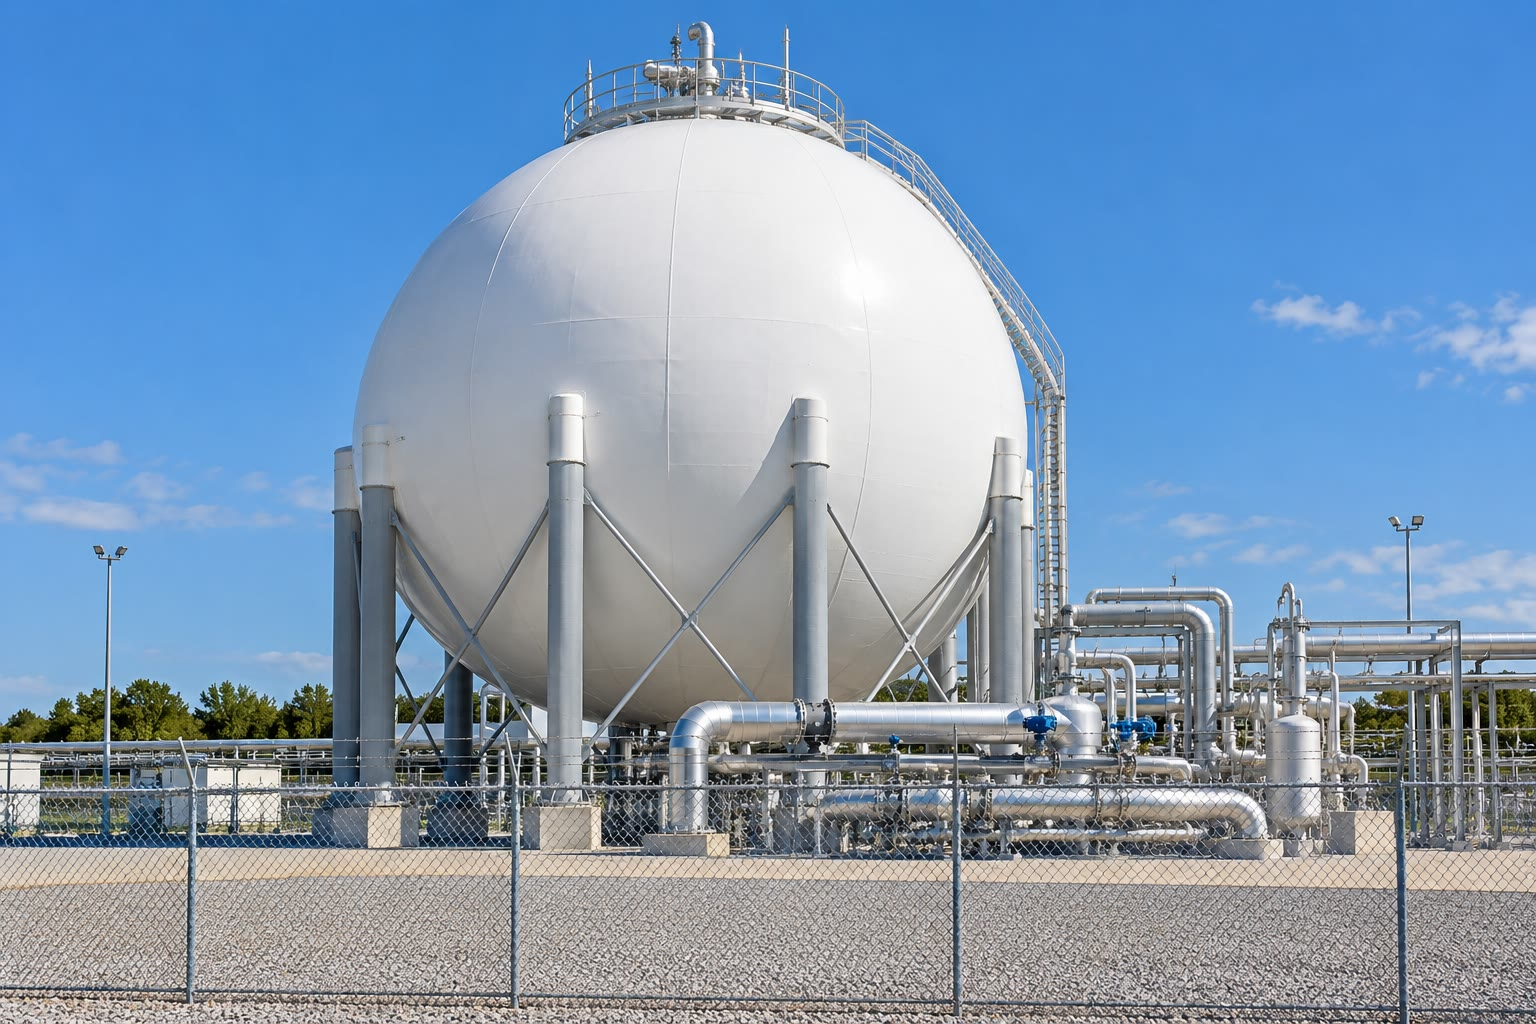
\includegraphics[width=0.6\linewidth]{images/book4/ai/b3-11-lh2-tank.jpg}

{\small Um tanque esférico de hidrogênio líquido. A \qty{20}{K}, o calor
produzido dentro do líquido pela lenta conversão de uma forma de spin nuclear
do hidrogênio na outra pode superar o calor que entra do exterior.}
\end{omfigure}

\section{Capacidades caloríficas dos gases}

A capacidade calorífica a volume constante é $C_V = (\partial U/\partial T)_V$, e,
pelo \cref{thm:b3:partition-functions:internal-energy}, cada tipo de movimento
contribui separadamente. Dois limites governam tudo.

\begin{theorem}[Teorema da equipartição]\label{thm:b3:statistical-thermo-applied:equipartition}
Quando os níveis de energia de um movimento são próximos em comparação com $kT$,
cada termo de sua energia quadrático em uma coordenada ou em um momento contribui
com $\frac12kT$ para a energia média de uma molécula, logo com $\frac12R$ para a
capacidade calorífica molar. Esse enunciado é o \emph{teorema da equipartição}\index{teorema da equiparticao@teorema da equipartição}.
\end{theorem}

\begin{proof}[Demonstração parcial]
No limite clássico, a soma sobre os estados de um movimento torna-se uma
integral, e um termo quadrático $a u^2$ contribui com o fator $\int\eu^{-\beta au^2}\dd u =
\sqrt{\pi/\beta a}$, proporcional a $\beta^{-1/2}$. Pelo
\cref{thm:b3:partition-functions:internal-energy}, sua energia média é
$-\partial\ln(\beta^{-1/2})/\partial\beta = 1/2\beta = \frac12kT$. Que a integral clássica seja o
limite da soma quântica foi mostrado para a translação e a rotação no
\cref{ch:b3:partition-functions}; para a vibração, decorre da proposição
seguinte quando $T \gg \theta_{\mathrm V}$.
\end{proof}

A translação tem três termos quadráticos ($\frac32R$); a rotação de uma molécula
linear, dois ($R$), a de uma não linear, três ($\frac32R$); cada vibração, dois,
cinético e potencial ($R$). Uma molécula linear de $N$ átomos tende, portanto, a
$C_{V,\mathrm m} = \frac52R + (3N - 5)R$ a alta temperatura. O limite quase nunca é
atingido para as vibrações à temperatura ambiente.

\begin{proposition}[Capacidade calorífica vibracional]\label{prop:b3:statistical-thermo-applied:cv-vib}
Uma vibração harmônica de temperatura característica $\theta_{\mathrm V}$ contribui com, sendo
$x = \theta_{\mathrm V}/T$,
\[
  \frac{C_{V,\mathrm m}^{\mathrm V}}{R} = \frac{x^2\eu^x}{(\eu^x - 1)^2},
\]
a função de Einstein, que tende a 1 quando $T \gg \theta_{\mathrm V}$ e cai
exponencialmente, como $x^2\eu^{-x}$, quando $T \ll \theta_{\mathrm V}$.
\end{proposition}

\begin{proof}
Pela \cref{prop:b3:partition-functions:q-vib}, $U - U(0) = R\theta_{\mathrm V}/(\eu^x - 1)$ por mol.
Derivando em relação a $T$, com $\dd x/\dd T = -x/T$, obtém-se
$R\theta_{\mathrm V}\eu^x(x/T)/(\eu^x - 1)^2 = Rx^2\eu^x/(\eu^x - 1)^2$. Para $x \to 0$, $\eu^x - 1 \approx x$ e a
razão tende a 1; para $x$ grande, ela se comporta como $x^2\eu^{-x}$.
\end{proof}

\begin{method}[A capacidade calorífica de um gás a partir de seus modos]\label{met:b3:statistical-thermo-applied:cv}
\begin{enumerate}
  \item Translação: $\frac32R$, sempre.
  \item Rotação: $R$ (linear) ou $\frac32R$ (não linear) se $T \gg \theta_{\mathrm R}$, o que vale para
        todo gás, exceto o hidrogênio, acima de algumas dezenas de kelvins.
  \item Vibrações: um termo de Einstein por \omterm{def:b3:group-theory-applied:normal-mode}{modo normal}, com $\theta_{\mathrm V} = hc\tilde\nu/k$ a partir
        dos números de onda fundamentais; um modo degenerado conta tantas vezes
        quanto sua \omterm{def:b3:quantum-model-systems:degenerate}{degenerescência}.
  \item Some, e $C_{p,\mathrm m} = C_{V,\mathrm m} + R$ para um gás ideal.
\end{enumerate}
\end{method}

Diz-se que um movimento está congelado quando $kT$ é pequeno diante de sua
primeira excitação: ele então não armazena energia e não contribui para $C_V$. A
vibração de \ce{N2} ($\theta_{\mathrm V} = \qty{3352}{K}$) está congelada à temperatura
ambiente e $C_{V,\mathrm m} = \frac52R$; a de \ce{Cl2} ($\theta_{\mathrm V} = \qty{798}{K}$) está
meio desperta, $C_{V,\mathrm m} = 3.07R$ a \qty{300}{K}.

\begin{omfigure}
\begin{tikzpicture}
\begin{axis}[width=0.86\linewidth, height=6.4cm, xmode=log, xmin=10, xmax=3000,
  ymin=1.3, ymax=3.9, axis lines=left, xlabel={$T$ / K}, ylabel={$C_{V,\mathrm m}/R$},
  tick label style={font=\small}, label style={font=\small},
  log ticks with fixed point, xtick={10,30,100,300,1000,3000},
  unbounded coords=jump]
\addplot[omDef, thick] table[x=T, y=N2] {figdata/out/bachelor-3-heat-capacity.dat};
\addplot[black!60, thick] table[x=T, y=Cl2] {figdata/out/bachelor-3-heat-capacity.dat};
\addplot[omThm, thick, dashed] table[x=T, y=nH2] {figdata/out/bachelor-3-heat-capacity.dat};
\addplot[omThm, thick] table[x=T, y=eH2] {figdata/out/bachelor-3-heat-capacity.dat};
\addplot[only marks, mark=*, mark size=1.6pt, omDef] table[x=T, y=N2] {figdata/out/bachelor-3-heat-capacity-janaf.dat};
\addplot[only marks, mark=square*, mark size=1.5pt, black!60] table[x=T, y=Cl2] {figdata/out/bachelor-3-heat-capacity-janaf.dat};
\draw[black!30, densely dotted] (axis cs:10,1.5) -- (axis cs:3000,1.5);
\draw[black!30, densely dotted] (axis cs:10,2.5) -- (axis cs:3000,2.5);
\draw[black!30, densely dotted] (axis cs:10,3.5) -- (axis cs:3000,3.5);
\node[font=\scriptsize, black!60, anchor=south east] at (axis cs:2900,1.5) {$\frac32$: transl.};
\node[font=\scriptsize, black!60, anchor=south west] at (axis cs:10.5,2.5) {$\frac52$: + rotação};
\node[font=\scriptsize, black!60, anchor=south west] at (axis cs:10.5,3.5) {$\frac72$: + vibração};
\node[font=\scriptsize, omThm, anchor=south west] at (axis cs:60,3.6) {\ce{H2} de equilíbrio};
\node[font=\scriptsize, omThm, anchor=north west] at (axis cs:130,1.78) {\ce{H2} normal};
\node[font=\scriptsize, black!70, anchor=south east] at (axis cs:560,3.33) {\ce{Cl2}};
\node[font=\scriptsize, omDef, anchor=south east] at (axis cs:1000,3.0) {\ce{N2}};
\end{axis}
\end{tikzpicture}

{\small Capacidade calorífica molar a volume constante, calculada a partir das
constantes espectroscópicas (linhas; \omterm{def:b3:quantum-model-systems:rotor}{rotor rígido}, vibração harmônica), com os
valores das tabelas termoquímicas para \ce{N2} e \ce{Cl2} (pontos, $C_p/R - 1$). A
vibração desperta perto de $\theta_{\mathrm V}/10$; acima de cerca de \qty{1000}{K}, as tabelas
sobem acima do modelo harmônico, que ignora a anarmonicidade. Hidrogênio: a
contribuição rotacional do hidrogênio normal (tracejada, orto e para congelados
em 3:1) e do hidrogênio de equilíbrio (contínua), que ultrapassa $\frac52$ porque
converter para em orto absorve calor.}
\end{omfigure}

\section{Estatística de spin nuclear}

Os dois núcleos de \ce{H2} são férmions idênticos. Permutá-los muda o sinal da
função de onda total (\cref{ch:b3:many-electron-atoms}); permutá-los equivale a
girar a molécula de ponta a ponta, o que multiplica a função de onda rotacional
$Y_{J,M}$ por $(-1)^J$ e a função de spin nuclear por $+1$ ou $-1$.

\begin{theorem}[Estatística de spin nuclear]\label{thm:b3:statistical-thermo-applied:spin-statistics}
Em uma molécula diatômica homonuclear cujos núcleos têm spin $I$, em um estado
eletrônico fundamental ${}^1\Sigma_g^+$, há $(2I+1)(I+1)$ estados de spin nuclear simétricos
e $(2I+1)I$ antissimétricos. Para os férmions ($I$ semi-inteiro), os antissimétricos
acompanham os $J$ pares e os simétricos os $J$ ímpares; para os bósons ($I$ inteiro),
o contrário. Para \ce{H2} ($I = \frac12$), os níveis pares e ímpares têm pesos de
spin 1 e 3; para \ce{D2} ($I = 1$), 6 e 3. Quando $I = 0$, só existe uma paridade de
$J$: a molécula linear de \ce{CO2}, com dois núcleos \ce{^{16}O} e um estado
fundamental simétrico, tem apenas níveis rotacionais pares.
\end{theorem}

\begin{proof}[Demonstração parcial]
O postulado de simetria (a função de onda total é antissimétrica na permutação
de dois férmions idênticos e simétrica para os bósons) é admitido. Os
$(2I+1)^2$ produtos de estados de spin de um núcleo $|m_1\rangle|m_2\rangle$ dão $2I+1$ estados
simétricos com $m_1 = m_2$ e, para cada um dos $(2I+1)2I/2$ pares $m_1 \ne m_2$, uma
combinação simétrica e uma antissimétrica: $(2I+1) + (2I+1)I = (2I+1)(I+1)$
estados simétricos e $(2I+1)I$ antissimétricos. Em um estado ${}^1\Sigma_g^+$, as funções
eletrônica e vibracional não mudam na permutação, de modo que o produto das
funções rotacional e de spin deve ter o sinal global exigido: para os
férmions, $(-1)^J \times(\text{simetria de spin}) = -1$, o que associa os $J$ pares
aos estados de spin antissimétricos. Para \ce{H2}: 3 simétricos, 1 antissimétrico;
para \ce{D2}: 6 e 3.
\end{proof}

\begin{definition}[Orto e para-hidrogênio]\label{def:b3:statistical-thermo-applied:spin-isomers}
O \emph{orto-hidrogênio}\index{orto-hidrogenio@orto-hidrogênio} é a forma de \ce{H2} com os spins
dos dois prótons em um estado simétrico (tripleto), que ocupa apenas os níveis
rotacionais ímpares; o \emph{para-hidrogênio}\index{para-hidrogenio@para-hidrogênio} é a forma com
o estado de spin antissimétrico (singleto), que ocupa apenas os níveis pares.
\end{definition}

Converter uma forma na outra exige inverter um spin nuclear em relação ao
outro, o que as colisões com outras moléculas de hidrogênio quase não fazem: no
hidrogênio puro, as duas formas se comportam durante dias como dois gases
diferentes. Uma superfície paramagnética, cujo campo magnético não homogêneo
age de modo diferente sobre os dois prótons, catalisa a conversão.

\begin{proposition}[Razão orto--para de equilíbrio]\label{prop:b3:statistical-thermo-applied:ortho-para}
No equilíbrio, a fração de \omterm{def:b3:statistical-thermo-applied:spin-isomers}{para-hidrogênio} é
\[
  x_{\mathrm{para}} = \frac{\sum_{J\,\mathrm{even}}(2J+1)\eu^{-\theta_{\mathrm R}J(J+1)/T}}
    {\sum_{J\,\mathrm{even}}(2J+1)\eu^{-\theta_{\mathrm R}J(J+1)/T} + 3\sum_{J\,\mathrm{odd}}(2J+1)\eu^{-\theta_{\mathrm R}J(J+1)/T}},
\]
que tende a 1 a 0 K e a $\frac14$ a alta temperatura. Para \ce{D2}, a forma orto
($J$ par) tende a 1 a 0 K e a $\frac23$ a alta temperatura.
\end{proposition}

\begin{proof}
A \omterm{def:b3:partition-functions:boltzmann}{distribuição de Boltzmann} sobre todos os estados, com os pesos de spin do
\cref{thm:b3:statistical-thermo-applied:spin-statistics}. A 0 K, só $J = 0$, que é
par, está povoado. A alta temperatura, as somas par e ímpar valem cada uma a
metade de $T/\theta_{\mathrm R}$, e a razão é $1 : 3$; para \ce{D2}, $6 : 3$.
\end{proof}

Para \ce{H2}, $\theta_{\mathrm R} = \qty{85.4}{K}$: a mistura de equilíbrio é metade para a \qty{78}{K},
99.8\,\% para no ponto de ebulição, \qty{20.37}{K}, e 25.07\,\% à temperatura
ambiente. O hidrogênio mantido à temperatura ambiente, chamado hidrogênio normal,
é portanto uma mistura 3:1 de orto e para.

\begin{omfigure}
\begin{tikzpicture}
\begin{axis}[width=0.72\linewidth, height=5.4cm, xmin=0, xmax=300, ymin=0, ymax=1.05,
  axis lines=left, xlabel={$T$ / K}, ylabel={fração de equilíbrio},
  tick label style={font=\small}, label style={font=\small}]
\addplot[omThm, thick] table[x=T, y=pH2] {figdata/out/bachelor-3-ortho-para.dat};
\addplot[omDef, thick] table[x=T, y=oD2] {figdata/out/bachelor-3-ortho-para.dat};
\draw[black!35, densely dotted] (axis cs:0,0.25) -- (axis cs:300,0.25);
\draw[black!35, densely dotted] (axis cs:0,0.6667) -- (axis cs:300,0.6667);
\node[font=\scriptsize, omThm, anchor=south west] at (axis cs:190,0.27) {fração para do \ce{H2} $\to \frac14$};
\node[font=\scriptsize, omDef, anchor=south west] at (axis cs:120,0.69) {fração orto do \ce{D2} $\to \frac23$};
\end{axis}
\end{tikzpicture}

{\small Composição de equilíbrio dos isômeros de spin nuclear em função da
temperatura, a partir dos níveis rotacionais e dos pesos de spin (\ce{H2}: 1 e 3;
\ce{D2}: 6 e 3). As duas formas com $J$ par predominam a baixa temperatura.}
\end{omfigure}

A capacidade calorífica do hidrogênio mostra as consequências. No hidrogênio
normal, as moléculas orto e para são dois gases misturados em proporções fixas;
cada um tem sua própria escada de níveis, começando em $J = 1$ e em $J = 0$, e sua
rotação congela separadamente. No hidrogênio de equilíbrio, o aquecimento também
converte para em orto, o que absorve energia e dá o pico da figura acima. As
primeiras medidas, feitas sem catalisador, seguiram a curva do hidrogênio
normal, e foi a interpretação dessa curva como uma mistura 3:1 congelada que
revelou pela primeira vez as duas formas.

\begin{remark}
O \omterm{def:b3:partition-functions:symmetry-number}{número de simetria} da \cref{prop:b3:partition-functions:q-rot} fica agora
justificado. A alta temperatura, cada estado de spin encontra permitida cerca da
metade dos níveis rotacionais, de modo que $\sum(\text{peso de spin})(2J+1)\eu^{\dots} \approx (2I+1)^2\,T/2\theta_{\mathrm R}$: o
fator de spin total $(2I+1)^2$ é deixado de fora por convenção, e resta $\sigma = 2$.
\end{remark}

\begin{definition}[Entropia residual]\label{def:b3:statistical-thermo-applied:residual-entropy}
A \emph{entropia residual}\index{entropia residual} de um cristal é a entropia que
ele conserva quando $T \to 0$ porque suas moléculas permanecem congeladas em um de
muitos arranjos de energia igual ou quase igual.
\end{definition}

\begin{proposition}[Entropias residuais do monóxido de carbono e do gelo]\label{prop:b3:statistical-thermo-applied:residual}
Um cristal de $N$ moléculas congelado em $W_0$ arranjos igualmente prováveis tem $S_0 =
k\ln W_0$. O \ce{CO} sólido, com cada molécula apontando para um lado ou para o outro,
tem $S_{0,\mathrm m} = R\ln2 =
\qty{5.76}{J.K^{-1}.mol^{-1}}$. O gelo, com cada oxigênio ligado a dois
átomos de hidrogênio e ligado por ligações de hidrogênio a outros dois, tem
$W_0 = (3/2)^N$ e $S_{0,\mathrm m} = R\ln\frac32 =
\qty{3.37}{J.K^{-1}.mol^{-1}}$.
\end{proposition}

\begin{proof}
A \cref{def:b3:partition-functions:statistical-entropy} aplicada para $T \to 0$.
\ce{CO}: o dipolo da molécula é tão pequeno que as orientações CO e OC têm quase
a mesma energia, e cada uma das $N$ moléculas tem duas: $W_0 = 2^N$, $S_0 = Nk\ln2$.
Gelo (contagem de Pauling): cada um dos $2N$ átomos de hidrogênio fica sobre uma
reta O$\cdots$O, perto de uma extremidade ou da outra: $2^{2N}$ arranjos. Das 16
maneiras de dispor os quatro hidrogênios em torno de um oxigênio, 6 lhe dão
exatamente dois hidrogênios próximos (uma molécula de água); tratando os oxigênios
como independentes, uma fração $6/16$ dos arranjos satisfaz cada um deles: $W_0 = 2^{2N}(6/16)^N = (3/2)^N$.
\end{proof}

As tabelas citam, para o \ce{CO}, a \omterm{def:b3:partition-functions:statistical-entropy}{entropia estatística}
(\cref{ch:b3:partition-functions}); o valor calorimétrico é mais baixo, com uma
diferença da ordem de $R\ln2$, um pouco menor porque as orientações não são
totalmente aleatórias. Para o gelo, a diferença entre a entropia calorimétrica do
vapor de água e seu valor estatístico concordou com a contagem de Pauling quando
ele a fez, em 1935, confirmando que os prótons do gelo são desordenados. O
terceiro princípio, na forma ``a entropia de um cristal perfeito é nula a 0 K'',
aplica-se aos cristais que chegam de fato a um único arranjo.

\begin{omfigure}
\begin{tikzpicture}[scale=1.15, every node/.style={transform shape}]
  \draw[black!45, dashed] (0.00,0.00) -- (1.20,0.00);
  \draw[black, thick] (0.00,0.00) -- (0.36,0.00); \node[aH, minimum size=2.2mm] at (0.36,0.00) {};
  \draw[black!45, dashed] (0.00,0.00) -- (0.00,1.20);
  \draw[black, thick] (0.00,0.00) -- (0.00,0.36); \node[aH, minimum size=2.2mm] at (0.00,0.36) {};
  \draw[black!45, dashed] (0.00,1.20) -- (1.20,1.20);
  \draw[black, thick] (0.00,1.20) -- (0.36,1.20); \node[aH, minimum size=2.2mm] at (0.36,1.20) {};
  \draw[black!45, dashed] (0.00,1.20) -- (0.00,2.40);
  \draw[black, thick] (0.00,2.40) -- (0.00,2.04); \node[aH, minimum size=2.2mm] at (0.00,2.04) {};
  \draw[black!45, dashed] (0.00,2.40) -- (1.20,2.40);
  \draw[black, thick] (1.20,2.40) -- (0.84,2.40); \node[aH, minimum size=2.2mm] at (0.84,2.40) {};
  \draw[black!45, dashed] (0.00,2.40) -- (0.00,3.60);
  \draw[black, thick] (0.00,3.60) -- (0.00,3.24); \node[aH, minimum size=2.2mm] at (0.00,3.24) {};
  \draw[black!45, dashed] (0.00,3.60) -- (1.20,3.60);
  \draw[black, thick] (1.20,3.60) -- (0.84,3.60); \node[aH, minimum size=2.2mm] at (0.84,3.60) {};
  \draw[black!45, dashed] (0.00,3.60) -- (0.00,4.20);
  \draw[black, thick] (0.00,3.60) -- (0.00,3.96); \node[aH, minimum size=2.2mm] at (0.00,3.96) {};
  \draw[black!45, dashed] (1.20,0.00) -- (2.40,0.00);
  \draw[black, thick] (1.20,0.00) -- (1.56,0.00); \node[aH, minimum size=2.2mm] at (1.56,0.00) {};
  \draw[black!45, dashed] (1.20,0.00) -- (1.20,1.20);
  \draw[black, thick] (1.20,1.20) -- (1.20,0.84); \node[aH, minimum size=2.2mm] at (1.20,0.84) {};
  \draw[black!45, dashed] (1.20,1.20) -- (2.40,1.20);
  \draw[black, thick] (2.40,1.20) -- (2.04,1.20); \node[aH, minimum size=2.2mm] at (2.04,1.20) {};
  \draw[black!45, dashed] (1.20,1.20) -- (1.20,2.40);
  \draw[black, thick] (1.20,1.20) -- (1.20,1.56); \node[aH, minimum size=2.2mm] at (1.20,1.56) {};
  \draw[black!45, dashed] (1.20,2.40) -- (2.40,2.40);
  \draw[black, thick] (1.20,2.40) -- (1.56,2.40); \node[aH, minimum size=2.2mm] at (1.56,2.40) {};
  \draw[black!45, dashed] (1.20,2.40) -- (1.20,3.60);
  \draw[black, thick] (1.20,3.60) -- (1.20,3.24); \node[aH, minimum size=2.2mm] at (1.20,3.24) {};
  \draw[black!45, dashed] (1.20,3.60) -- (2.40,3.60);
  \draw[black, thick] (2.40,3.60) -- (2.04,3.60); \node[aH, minimum size=2.2mm] at (2.04,3.60) {};
  \draw[black!45, dashed] (1.20,3.60) -- (1.20,4.20);
  \draw[black!45, dashed] (2.40,0.00) -- (3.60,0.00);
  \draw[black, thick] (3.60,0.00) -- (3.24,0.00); \node[aH, minimum size=2.2mm] at (3.24,0.00) {};
  \draw[black!45, dashed] (2.40,0.00) -- (2.40,1.20);
  \draw[black, thick] (2.40,0.00) -- (2.40,0.36); \node[aH, minimum size=2.2mm] at (2.40,0.36) {};
  \draw[black!45, dashed] (2.40,1.20) -- (3.60,1.20);
  \draw[black, thick] (2.40,1.20) -- (2.76,1.20); \node[aH, minimum size=2.2mm] at (2.76,1.20) {};
  \draw[black!45, dashed] (2.40,1.20) -- (2.40,2.40);
  \draw[black, thick] (2.40,2.40) -- (2.40,2.04); \node[aH, minimum size=2.2mm] at (2.40,2.04) {};
  \draw[black!45, dashed] (2.40,2.40) -- (3.60,2.40);
  \draw[black, thick] (3.60,2.40) -- (3.24,2.40); \node[aH, minimum size=2.2mm] at (3.24,2.40) {};
  \draw[black!45, dashed] (2.40,2.40) -- (2.40,3.60);
  \draw[black, thick] (2.40,2.40) -- (2.40,2.76); \node[aH, minimum size=2.2mm] at (2.40,2.76) {};
  \draw[black!45, dashed] (2.40,3.60) -- (3.60,3.60);
  \draw[black, thick] (2.40,3.60) -- (2.76,3.60); \node[aH, minimum size=2.2mm] at (2.76,3.60) {};
  \draw[black!45, dashed] (2.40,3.60) -- (2.40,4.20);
  \draw[black!45, dashed] (3.60,0.00) -- (4.20,0.00);
  \draw[black, thick] (3.60,0.00) -- (3.96,0.00); \node[aH, minimum size=2.2mm] at (3.96,0.00) {};
  \draw[black!45, dashed] (3.60,0.00) -- (3.60,1.20);
  \draw[black, thick] (3.60,1.20) -- (3.60,0.84); \node[aH, minimum size=2.2mm] at (3.60,0.84) {};
  \draw[black!45, dashed] (3.60,1.20) -- (4.20,1.20);
  \draw[black!45, dashed] (3.60,1.20) -- (3.60,2.40);
  \draw[black, thick] (3.60,1.20) -- (3.60,1.56); \node[aH, minimum size=2.2mm] at (3.60,1.56) {};
  \draw[black!45, dashed] (3.60,2.40) -- (4.20,2.40);
  \draw[black!45, dashed] (3.60,2.40) -- (3.60,3.60);
  \draw[black, thick] (3.60,2.40) -- (3.60,2.76); \node[aH, minimum size=2.2mm] at (3.60,2.76) {};
  \draw[black!45, dashed] (3.60,3.60) -- (4.20,3.60);
  \draw[black, thick] (3.60,3.60) -- (3.96,3.60); \node[aH, minimum size=2.2mm] at (3.96,3.60) {};
  \draw[black!45, dashed] (3.60,3.60) -- (3.60,4.20);
  \draw[black, thick] (3.60,3.60) -- (3.60,3.96); \node[aH, minimum size=2.2mm] at (3.60,3.96) {};
  \draw[black!45, dashed] (-0.60,0.00) -- (0.00,0.00);
  \draw[black!45, dashed] (-0.60,1.20) -- (0.00,1.20);
  \draw[black, thick] (0.00,1.20) -- (-0.36,1.20); \node[aH, minimum size=2.2mm] at (-0.36,1.20) {};
  \draw[black!45, dashed] (-0.60,2.40) -- (0.00,2.40);
  \draw[black, thick] (0.00,2.40) -- (-0.36,2.40); \node[aH, minimum size=2.2mm] at (-0.36,2.40) {};
  \draw[black!45, dashed] (-0.60,3.60) -- (0.00,3.60);
  \draw[black!45, dashed] (0.00,-0.60) -- (0.00,0.00);
  \draw[black!45, dashed] (1.20,-0.60) -- (1.20,0.00);
  \draw[black, thick] (1.20,0.00) -- (1.20,-0.36); \node[aH, minimum size=2.2mm] at (1.20,-0.36) {};
  \draw[black!45, dashed] (2.40,-0.60) -- (2.40,0.00);
  \draw[black, thick] (2.40,0.00) -- (2.40,-0.36); \node[aH, minimum size=2.2mm] at (2.40,-0.36) {};
  \draw[black!45, dashed] (3.60,-0.60) -- (3.60,0.00);
  \node[aO, minimum size=4mm] at (0.00,0.00) {};
  \node[aO, minimum size=4mm] at (0.00,1.20) {};
  \node[aO, minimum size=4mm] at (0.00,2.40) {};
  \node[aO, minimum size=4mm] at (0.00,3.60) {};
  \node[aO, minimum size=4mm] at (1.20,0.00) {};
  \node[aO, minimum size=4mm] at (1.20,1.20) {};
  \node[aO, minimum size=4mm] at (1.20,2.40) {};
  \node[aO, minimum size=4mm] at (1.20,3.60) {};
  \node[aO, minimum size=4mm] at (2.40,0.00) {};
  \node[aO, minimum size=4mm] at (2.40,1.20) {};
  \node[aO, minimum size=4mm] at (2.40,2.40) {};
  \node[aO, minimum size=4mm] at (2.40,3.60) {};
  \node[aO, minimum size=4mm] at (3.60,0.00) {};
  \node[aO, minimum size=4mm] at (3.60,1.20) {};
  \node[aO, minimum size=4mm] at (3.60,2.40) {};
  \node[aO, minimum size=4mm] at (3.60,3.60) {};
\end{tikzpicture}

{\small A desordem dos prótons no gelo, desenhada como uma rede quadrada plana (a
rede real é tetraédrica): cada oxigênio (vermelho) tem quatro vizinhos O$\cdots$O,
um hidrogênio (branco) em cada reta, e exatamente dois hidrogênios próximos dele
(as regras do gelo). Este é um dos $(3/2)^N$ arranjos da contagem de Pauling; todos
eles têm quase a mesma energia, e o congelamento escolhe um ao acaso.}
\end{omfigure}

\section{Constantes de equilíbrio a partir das funções de partição}

\begin{theorem}[Constante de equilíbrio a partir das funções de partição]\label{thm:b3:statistical-thermo-applied:k-from-q}
Para uma reação $0 = \sum_J\nu_J\mathrm J$ entre gases ideais,
\[
  K^\circ = \prod_J\Bigl(\frac{q^\circ_{J,\mathrm m}}{N_A}\Bigr)^{\nu_J}\eu^{-\Delta_rE_0/RT},
\]
onde $q^\circ_{J,\mathrm m}$ é a função de partição de $\mathrm J$ no volume molar padrão
$V^\circ_{\mathrm m} = RT/p^\circ$, cada uma contada a partir de seu próprio estado fundamental, e $\Delta_rE_0 =
\sum\nu_JE_{0,J}$ é a energia molar de reação a 0 K, do estado fundamental dos
reagentes ao dos produtos.
\end{theorem}

\begin{proof}
Pelo \cref{thm:b3:partition-functions:entropy}, um mol de gás ideal $\mathrm J$ a $p^\circ$ tem
$G^\circ_{\mathrm m} - G_{\mathrm m}(0) = -RT\ln(q^\circ_{J,\mathrm m}/N_A)$, e $G_{\mathrm m}(0)$ é a energia $E_{0,J}$
de seu estado fundamental em uma escala comum a todas as espécies. Logo $\Delta_rG^\circ =
\Delta_rE_0 - RT\sum_J\nu_J\ln(q^\circ_{J,\mathrm m}/N_A)$, e $\Delta_rG^\circ = -RT\ln K^\circ$ dá o
resultado.
\end{proof}

\begin{method}[Calcular uma constante de equilíbrio a partir de dados espectroscópicos]\label{met:b3:statistical-thermo-applied:k-stat}
\begin{enumerate}
  \item Para cada espécie: $q^\circ_{\mathrm m}/N_A = (kT/p^\circ)\Lambda^{-3}\times q^{\mathrm R}q^{\mathrm V}q^{\mathrm E}$, com os
        \omterm{def:b3:partition-functions:symmetry-number}{números de simetria} e as \omterm{def:b3:quantum-model-systems:degenerate}{degenerescências} eletrônicas.
  \item $\Delta_rE_0$ a partir das energias de dissociação $D_0$ (medidas a partir do
        nível vibracional fundamental, de modo que as \omterm{def:b3:quantum-model-systems:oscillator}{energias do ponto zero} estão
        incluídas) ou das entalpias de formação a 0 K.
  \item Multiplique e verifique as unidades: $K^\circ$ é um número puro, e a pressão
        padrão entra por meio de $kT/p^\circ$.
\end{enumerate}
\end{method}

\begin{example}[A dissociação do iodo]\label{ex:b3:statistical-thermo-applied:iodine}
% ledger: janaf:I.dfH0, janaf:I2g.dfH0, lev:I.2P1_2, diat:I2.we, diat:I2.wexe, diat:I2.Be, diat:I2.ae, aw:I, janaf:I.logKf.1000
Para $\ce{I2(g) <=> 2 I(g)}$, $\Delta_rE_0 = D_0(\ce{I2}) = 2 \times 107.164 - 65.504 = \qty{148.824}{kJ/mol}$
a partir das entalpias de formação a 0 K das tabelas termoquímicas. A
\qty{1000}{K}: para I, $\Lambda = \qty{4.90}{pm}$, $kT/p^\circ = \qty{1.381e-25}{m^3}$, $q^{\mathrm E} = 4 +
2\eu^{-10.94} = 4.0000$ (o nível ${}^2P_{1/2}$ fica \qty{7603}{cm^{-1}} acima), logo $q^\circ_{\mathrm m}/N_A = \num{4.69e9}$;
para \ce{I2}, $\Lambda = \qty{3.47}{pm}$, $q^{\mathrm R} = 1000/(2 \times 0.05369) = 9313$ e $q^{\mathrm V} = 3.784$, logo
$q^\circ_{\mathrm m}/N_A = \num{1.17e14}$. Então $K^\circ = (4.69\times10^9)^2/(1.17\times10^{14}) \times \eu^{-17.90} =
\num{3.17e-3}$, $\log K^\circ = -2.50$; as tabelas dão $-2.51$.
\end{example}

\begin{omfigure}
\begin{tikzpicture}
\begin{axis}[name=ki, width=0.5\linewidth, height=5.6cm, xmin=0.58, xmax=1.45, ymin=-6.5,
  ymax=1, axis lines=left, xlabel={$1000\,\mathrm K/T$}, ylabel={$\log K^\circ$},
  tick label style={font=\small}, label style={font=\small},
  title={\small $\ce{I2 <=> 2 I}$}]
\addplot[black, thick] table[x=invT, y=logK] {figdata/out/bachelor-3-equilibrium-constant-stat-i2.dat};
\addplot[only marks, mark=*, mark size=1.8pt, omThm] table[x=invT, y=logK] {figdata/out/bachelor-3-equilibrium-constant-stat-i2-janaf.dat};
\node[font=\scriptsize, anchor=north east, align=right] at (axis cs:1.43,0.8) {linha: estatística\\ pontos: tabelas};
\end{axis}
\begin{axis}[at={(ki.east)}, anchor=west, xshift=1.4cm, width=0.44\linewidth, height=5.6cm,
  xmin=0, xmax=2000, ymin=0, ymax=4.4, axis lines=left, xlabel={$T$ / K},
  ylabel={$K^\circ$}, tick label style={font=\small}, label style={font=\small},
  title={\small $\ce{H2 + D2 <=> 2 HD}$}, scaled x ticks=false,
  xticklabel style={/pgf/number format/1000 sep={}}]
\addplot[omDef, thick] table[x=T, y=K] {figdata/out/bachelor-3-equilibrium-constant-stat-hd.dat};
\draw[black!35, densely dotted] (axis cs:0,4) -- (axis cs:2000,4);
\node[font=\scriptsize, anchor=north east] at (axis cs:1950,3.95) {limite de $\sigma$: 4};
\end{axis}
\end{tikzpicture}

{\small Constantes de equilíbrio calculadas a partir das funções de partição. À
esquerda: a dissociação do iodo, uma reta de van 't Hoff de inclinação $-\Delta_rH^\circ/(R\ln10)$,
com os valores das tabelas termoquímicas (pontos). À direita: a troca $\ce{H2 + D2
<=> 2 HD}$, que tende à razão dos \omterm{def:b3:partition-functions:symmetry-number}{números de simetria}, 4, a alta temperatura e
fica abaixo dela a baixa temperatura por causa das \omterm{def:b3:quantum-model-systems:oscillator}{energias do ponto zero} e das
restrições de spin nuclear.}
\end{omfigure}

\begin{proposition}[A troca H$_2$ + D$_2$]\label{prop:b3:statistical-thermo-applied:hd}
Para $\ce{H2 + D2 <=> 2 HD}$, $K^\circ \to 4$ a alta temperatura.
\end{proposition}

\begin{proof}
A alta temperatura, os fatores translacional, rotacional e vibracional são
$m^{3/2}$, $T/\sigma\theta_{\mathrm R} \propto \mu/\sigma$ e $T/\theta_{\mathrm V} \propto \sqrt\mu$ (a \omterm{def:b3:quantum-model-systems:oscillator}{constante de força},
propriedade eletrônica, é a mesma para as três moléculas), e $\Delta_rE_0/RT \to 0$.
Com $m_{\ce{H2}} = 2$, $m_{\ce{D2}} = 4$, $m_{\ce{HD}} = 3$ e $\mu = 1/2$, 1, $2/3$ (em unidades da
massa do próton, ignorando a pequena diferença entre D e 2H):
\[
  K^\circ \to \Bigl(\frac{9}{8}\Bigr)^{3/2} \times \frac{(2/3)^2/1^2}{(1/2)(1)/(2 \times 2)}
  \times \frac{2/3}{\sqrt{1/2}\sqrt1}
  = \frac{27}{16\sqrt2} \times \frac{32}{9} \times \frac{2\sqrt2}{3} = 4 .
\]
Todos os fatores de massa se cancelam exatamente: só restam os \omterm{def:b3:partition-functions:symmetry-number}{números de simetria}, $\sigma_{\ce{H2}}
\sigma_{\ce{D2}}/\sigma_{\ce{HD}}^2 = 4$.
\end{proof}

A \qty{298.15}{K}, a constante estatística vale 3.26: as \omterm{def:b3:quantum-model-systems:oscillator}{energias do ponto zero} de \ce{H2},
\ce{D2} e HD (\qty{2170.3}{cm^{-1}}, \qty{1542.3}{cm^{-1}} e \qty{1883.7}{cm^{-1}}) dão $\Delta_rE_0 =
\qty{54.8}{cm^{-1}}$, um fator $\eu^{-54.8/207.2} = 0.77$; a rotação, ainda parcialmente
quantizada para essas moléculas leves, também importa.

\begin{proposition}[A equação de van 't Hoff reencontrada]\label{prop:b3:statistical-thermo-applied:vant-hoff-stat}
A constante de equilíbrio estatística obedece a $\dfrac{\dd\ln K^\circ}{\dd T} = \dfrac{\Delta_rH^\circ}{RT^2}$.
\end{proposition}

\begin{proof}
Cada $q^\circ_{J,\mathrm m}$ depende de $T$ por seus níveis e por $V^\circ_{\mathrm m} = RT/p^\circ$:
$\dd\ln q^\circ_{J,\mathrm m}/\dd T = (U_J - U_J(0))/RT^2 + 1/T$ por mol, pelo
\cref{thm:b3:partition-functions:internal-energy}. Logo $\dd\ln K^\circ/\dd T =
[\Delta_rE_0 + \sum\nu_J(U_J - U_J(0)) + \sum\nu_JRT]/RT^2 = (\Delta_rU + \Delta\nu_{\mathrm g}RT)/RT^2 =
\Delta_rH^\circ/RT^2$ para gases ideais.
\end{proof}

Da inclinação do painel esquerdo da figura, a entalpia de dissociação do iodo
perto de \qty{1000}{K} é \qty{154}{kJ/mol}: $D_0$ mais a energia translacional
extra de dois átomos em relação a uma molécula, menos a energia rotacional e
vibracional desta.

\section{Efeitos isotópicos}

Os \omterm{def:b3:rovibrational-spectroscopy:rotational-constant}{isotopólogos} têm a mesma estrutura eletrônica, logo a mesma curva de energia
potencial e as mesmas \omterm{def:b3:quantum-model-systems:oscillator}{constantes de força}, mas massas diferentes: seus números de
onda vibracionais, suas \omterm{def:b3:quantum-model-systems:oscillator}{energias do ponto zero} e suas funções de partição diferem,
assim como suas constantes de equilíbrio.

\begin{definition}[Efeito isotópico de equilíbrio, fator de fracionamento, valor $\delta$]\label{def:b3:statistical-thermo-applied:isotope-effect}
O \emph{efeito isotópico de equilíbrio}\index{efeito isotopico de equilibrio@efeito isotópico de equilíbrio} de uma
reação é a razão $K_{\mathrm{light}}/K_{\mathrm{heavy}}$ de suas constantes de equilíbrio com o
isótopo leve e com o pesado. O \emph{fator de fracionamento}\index{fator de fracionamento}
entre duas fases ou compostos A e B é $\alpha_{\mathrm{A/B}} = R_{\mathrm A}/R_{\mathrm B}$, onde
$R$ é a razão entre o isótopo pesado e o leve (por exemplo, $\ce{^{18}O}/\ce{^{16}O}$). O
\emph{valor $\delta$}\index{valor delta@valor $\delta$} de uma amostra é $\delta = (R_{\mathrm{sample}}/R_{\mathrm{standard}}
- 1) \times 1000$, em por mil (\textperthousand).
\end{definition}

\begin{proposition}[Efeitos isotópicos a partir das energias do ponto zero]\label{prop:b3:statistical-thermo-applied:zpe-isotope}
Para uma troca $\ce{XH + YD <=> XD + YH}$ a temperaturas em que as vibrações de
estiramento estão congeladas, o fator dominante da constante de equilíbrio é
\[
  K \approx \exp\Bigl(-\frac{\Delta\mathrm{ZPE}}{kT}\Bigr), \qquad
  \Delta\mathrm{ZPE} = \tfrac12hc\bigl[\tilde\nu_{\mathrm{XD}} + \tilde\nu_{\mathrm{YH}} - \tilde\nu_{\mathrm{XH}} - \tilde\nu_{\mathrm{YD}}\bigr],
\]
e $\tilde\nu_{\mathrm D} \approx \tilde\nu_{\mathrm H}/\sqrt2$ para um hidrogênio ligado a um átomo pesado. O isótopo
pesado se concentra na ligação mais rígida.
\end{proposition}

\begin{proof}
O \cref{thm:b3:statistical-thermo-applied:k-from-q} com as energias medidas a
partir do fundo das curvas de potencial comuns: $\Delta_rE_0$ é a variação da
\omterm{def:b3:quantum-model-systems:oscillator}{energia do ponto zero}. Os fatores translacional e rotacional quase se cancelam
entre duas trocas dos mesmos isótopos em parceiros pesados, e as funções de
partição vibracionais valem 1 quando congeladas. Com $\tilde\nu \propto \mu^{-1/2}$ e
$\mu_{\mathrm{XD}} \approx 2\mu_{\mathrm{XH}}$ para X pesado, $\tilde\nu_{\mathrm{XD}} = \tilde\nu_{\mathrm{XH}}/\sqrt2$, e $\Delta\mathrm{ZPE} =
\frac12hc(1 - 1/\sqrt2)(\tilde\nu_{\mathrm{YH}} - \tilde\nu_{\mathrm{XH}})$: negativa, logo $K > 1$, quando X--H é a
ligação mais rígida.
\end{proof}

O mesmo raciocínio explica o fracionamento dos isótopos do oxigênio entre a
água e seu vapor, entre a água e o carbonato de uma concha, ou entre dois
minerais: o \omterm{def:b3:statistical-thermo-applied:isotope-effect}{fator de fracionamento} tende a 1 a alta temperatura (assim como
$K_{\mathrm{HD}}$ tende a seu limite de simetria) e se afasta de 1 quando a temperatura
cai. Medido como valores $\delta$, ele é um termômetro: o $\delta^{18}$O do carbonato
das conchas fósseis registra a temperatura da água em que elas cresceram, e o do
gelo dos testemunhos polares, a temperatura das nuvens que formaram sua neve.

\begin{inthelab}[Um conversor orto--para]
Um liquefator de hidrogênio resfria o gás em etapas e, entre as etapas, o faz
passar por leitos de um catalisador paramagnético, tipicamente óxido de
ferro(III) hidratado. O calor de conversão é então removido em cada temperatura
pelo refrigerador, e o líquido que chega ao tanque está próximo de sua composição
de equilíbrio, quase inteiramente para. Sem o catalisador, o calor de conversão
seria liberado no tanque.
\end{inthelab}

\begin{safety}{\ghs[0.8cm]{GHS02}\ghs[0.8cm]{GHS04}}
% ledger: ghs:H2
Hidrogênio: gás extremamente inflamável, armazenado sob pressão ou como líquido
criogênico. Forma misturas explosivas com o ar em uma faixa muito ampla e queima
com uma chama quase invisível; o líquido causa queimaduras pelo frio e seu
vapor desloca o ar.
\end{safety}

\begin{history}[Os dois hidrogênios, 1927--1929]
Werner Heisenberg e Friedrich Hund previram em 1927 que as moléculas de
hidrogênio deveriam existir em duas formas que diferem por seus spins nucleares,
e David Dennison mostrou no mesmo ano que a intrigante capacidade calorífica do
hidrogênio medida abaixo da temperatura ambiente era a de uma mistura 3:1 das
duas, congelada em sua composição da temperatura ambiente. Em 1929, Karl
Friedrich Bonhoeffer e Paul Harteck adsorveram hidrogênio em carvão à temperatura
do ar líquido, dessorveram \omterm{def:b3:statistical-thermo-applied:spin-isomers}{para-hidrogênio} quase puro, reconhecido por sua
condutividade térmica diferente, e constataram que ele só voltava à mistura
normal muito lentamente.
\end{history}

\section{Exercícios}

\begin{exercise}[$\star$]\label{exo:b3:statistical-thermo-applied:1}
Dê o limite de alta temperatura de $C_{V,\mathrm m}$ do \ce{CO2} (linear, 3 átomos) e diga
quais contribuições ainda estão congeladas à temperatura ambiente.
\end{exercise}

\begin{exercise}[$\star$]\label{exo:b3:statistical-thermo-applied:2}
Avalie a função de Einstein em $T = \theta_{\mathrm V}$ e em $T = \theta_{\mathrm V}/10$.
\end{exercise}

\begin{exercise}[$\star$]\label{exo:b3:statistical-thermo-applied:3}
% ledger: diat:H2.Be, diat:H2.ae
Com $\theta_{\mathrm R} = \qty{85.35}{K}$ para \ce{H2}, calcule a fração para de equilíbrio a
\qty{20}{K} (só importam $J = 0$ e $J = 1$) e a \qty{77}{K} ($J \le 3$).
\end{exercise}

\begin{exercise}[$\star$]\label{exo:b3:statistical-thermo-applied:4}
Explique por que o deutério (spin nuclear 1) dá os pesos orto:para $6 : 3$, que
forma é estável a 0 K e qual é a razão à temperatura ambiente.
\end{exercise}

\begin{exercise}[$\star\star$]\label{exo:b3:statistical-thermo-applied:5}
% ledger: diat:H2.we, diat:H2.wexe, diat:D2.we, diat:D2.wexe, diat:HD.we, diat:HD.wexe
As \omterm{def:b3:quantum-model-systems:oscillator}{energias do ponto zero} de \ce{H2}, \ce{D2} e HD são 2170.3, 1542.3 e
\qty{1883.7}{cm^{-1}}. Calcule $\Delta_rE_0$ para $\ce{H2 + D2 <=> 2 HD}$ e o fator $\eu^{-\Delta_rE_0/RT}$ a
\qty{298.15}{K}. Compare $4\eu^{-\Delta_rE_0/RT}$ com o valor estatístico completo, 3.26.
\end{exercise}

\begin{exercise}[$\star\star$]\label{exo:b3:statistical-thermo-applied:6}
Estime a \omterm{def:b3:statistical-thermo-applied:residual-entropy}{entropia residual} de um cristal de \ce{N2O} (NNO linear, que pode
apontar para um lado ou para o outro) e de \ce{CH3D} (que pode pôr seu D em
qualquer uma de quatro posições).
\end{exercise}

\begin{exercise}[$\star\star$]\label{exo:b3:statistical-thermo-applied:7}
% ledger: diat:Cl2.we, diat:Cl2.wexe, janaf:Cl2.Cp.300
Calcule a $C_{p,\mathrm m}$ do \ce{Cl2} a \qty{300}{K} a partir de $\theta_{\mathrm V} = \qty{797.6}{K}$ e compare com o
valor tabelado \qty{33.981}{J.K^{-1}.mol^{-1}}.
\end{exercise}

\begin{exercise}[$\star\star$]\label{exo:b3:statistical-thermo-applied:8}
% ledger: diat:I2.we, diat:I2.wexe
Calcule a capacidade calorífica vibracional do \ce{I2} ($\theta_{\mathrm V} = \qty{306.9}{K}$) a
\qty{298.15}{K}, como fração de seu valor de equipartição.
\end{exercise}

\begin{exercise}[$\star\star$]\label{exo:b3:statistical-thermo-applied:9}
Uma amostra de água A tem $\delta^{18}\mathrm O = -10.0$\,\textperthousand\ e uma amostra B,
$+2.0$\,\textperthousand\ na mesma escala. Qual é mais rica em \ce{^{18}O}? Calcule o
\omterm{def:b3:statistical-thermo-applied:isotope-effect}{fator de fracionamento} $\alpha_{\mathrm{A/B}}$.
\end{exercise}

\begin{exercise}[$\star\star\star$]\label{exo:b3:statistical-thermo-applied:10}
Na troca $\ce{XH + YD <=> XD + YH}$ (dados do exercício), $\tilde\nu_{\mathrm{XH}} =
\qty{3000}{cm^{-1}}$ e $\tilde\nu_{\mathrm{YH}} = \qty{2000}{cm^{-1}}$, com X e Y pesados. Estime $K$ a
\qty{298.15}{K} e diga para onde vai o deutério.
\end{exercise}

\begin{exercise}[$\star\star\star$]\label{exo:b3:statistical-thermo-applied:11}
% ledger: janaf:I.dfH0, janaf:I2g.dfH0, lev:I.2P1_2, diat:I2.we, diat:I2.wexe, diat:I2.Be, diat:I2.ae, aw:I
As constantes estatísticas de $\ce{I2 <=> 2 I}$ são $\log K^\circ = -3.392$ a \qty{900}{K} e
$-1.766$ a \qty{1100}{K}. Deduza o $\Delta_rH^\circ$ médio no intervalo e explique
por que ele excede $D_0 = \qty{148.8}{kJ/mol}$.
\end{exercise}

\begin{exercise}[$\star\star\star$]\label{exo:b3:statistical-thermo-applied:12}
Para o \omterm{def:b3:statistical-thermo-applied:spin-isomers}{para-hidrogênio} a baixa temperatura, só importam $J = 0$ e $J = 2$. Mostre que
sua capacidade calorífica rotacional é $C/R = 5x^2\eu^{-x}/(1 + 5\eu^{-x})^2$ com $x = 6\theta_{\mathrm R}/T$, e
avalie-a a \qty{100}{K} ($\theta_{\mathrm R} = \qty{85.35}{K}$).
\end{exercise}

\section{Problema: Armazenar hidrogênio líquido}

\begin{problem}[{Problema de fim de semana --- armazenar hidrogênio líquido: as duas
formas de spin nuclear, o calor de sua conversão, a evaporação que ele provoca e
o catalisador que a impede}]
\label{pb:b3:statistical-thermo-applied:1}
% ledger: diat:H2.Be, diat:H2.ae, diat:H2.De, hvap:nH2, tb:nH2, aw:H
O hidrogênio é liquefeito em seu ponto de ebulição, \qty{20.37}{K} sob \qty{1.01325}{bar}, onde sua
entalpia de vaporização é \qty{0.905}{kJ/mol}. Níveis rotacionais: $F(J) = B_0J(J+1) -
D J^2(J+1)^2$ com $B_0 = \qty{59.322}{cm^{-1}}$ e $D = \qty{0.0471}{cm^{-1}}$ ($\theta_{\mathrm R} = \qty{85.35}{K}$).
Massa molar \qty{2.016}{g/mol}. A conversão orto $\to$ para não catalisada no líquido
é tomada como de primeira ordem, $k = \qty{0.0114}{h^{-1}}$ (dados do problema).

\medskip\noindent\textbf{Parte I --- As duas formas.}
\begin{enumerate}
  \item Quantos estados de spin nuclear tem um par de prótons? Quantos são
        simétricos na permutação, quantos antissimétricos?
  \item Quais estados de spin acompanham os $J$ pares, quais os $J$ ímpares, e por quê?
  \item Dê os pesos de spin dos níveis pares e ímpares.
  \item Mostre que a razão orto:para do hidrogênio à temperatura ambiente é 3:1.
  \item Calcule a energia de $J = 1$ acima de $J = 0$, em \unit{cm^{-1}} e em
        \unit{kJ/mol}.
  \item Calcule a fração para de equilíbrio a \qty{20.37}{K}.
  \item A mistura de equilíbrio é metade para a cerca de \qty{78}{K}. Por que essa
        temperatura é próxima de $\theta_{\mathrm R}$?
\end{enumerate}

\medskip\noindent\textbf{Parte II --- O calor de conversão.}
\begin{enumerate}[resume]
  \item Qual é a fração orto do hidrogênio recém-liquefeito sem catalisador? Por
        que ela não muda durante a liquefação?
  \item Calcule o calor liberado quando um mol dele atinge o equilíbrio a
        \qty{20.37}{K}.
  \item Exprima-o por quilograma.
  \item Exprima a entalpia de vaporização por quilograma.
  \item Compare os dois.
  \item Por que um isolamento melhor do tanque não pode eliminar esse calor?
\end{enumerate}

\medskip\noindent\textbf{Parte III --- A evaporação.}
\begin{enumerate}[resume]
  \item Dê a fração orto depois de um tempo $t$ no tanque.
  \item Calcule-a depois de \qty{24}{h}.
  \item Calcule o calor liberado por mol de líquido nas primeiras \qty{24}{h}.
  \item Que fração do líquido esse calor evaporaria?
  \item Repita para uma semana. Por que essa estimativa simples exagera a perda?
  \item Calcule o tempo de meia-vida da conversão.
\end{enumerate}

\medskip\noindent\textbf{Parte IV --- O catalisador e a capacidade calorífica.}
\begin{enumerate}[resume]
  \item Onde, em um liquefator, a conversão deve ocorrer, e por quê?
  \item O hidrogênio normal a \qty{300}{K} está em equilíbrio orto--para?
  \item Por que os hidrogênios normal e de equilíbrio têm capacidades caloríficas
        diferentes entre cerca de 30 e \qty{200}{K}?
  \item Leia na figura da capacidade calorífica o máximo de $C_{V,\mathrm m}/R$ do
        hidrogênio de equilíbrio e explique por que ele excede $\frac52$.
  \item Quanto vale a $C_{V,\mathrm m}/R$ do hidrogênio normal a \qty{50}{K}?
  \item Enuncie o resultado: a razão entre o calor de conversão do hidrogênio normal
        e sua entalpia de vaporização, e seu significado para o tanque.
\end{enumerate}
\end{problem}
